\section{Theory}

Conceptually these systems are quite simple to model,
consisting of binary spins which can either have the value 1 (up) or -1 (down).
The energy of this system is given by summing up nearest neighbour spins of all
the spins in our system. We evolve our system by randomly selecting spins and
changing their values if it is energetically favourable for the system. To not
have our system being stuck in the ground state (lowest energy state) we will
follow the Metropolis algorithm to randomly flip some spins anyway, a
behaviour is which seen for real systems.


\subsection{Ising model}
The Ising model, without an external magnetic field, is given by
\cref{eq:ising}, where $E_i$ is the energy of a given microstate s$_k$ and s$_l$ takes values of $\pm 1$, O is the
number of spins, J is a coupling constant corresponding to the strength of the
interaction between the neighbouring spins and $<kl>$ means that we sum over
nearest neighbour only.

\begin{equation}\label{eq:ising}
  E_i = -J\sum_{<kl>}^{O} s_k s_l
\end{equation}
The parameter that we can control in our experiment is the temperature, and it
is therefore it is natural to
use the canonical ensemble where temperature is the intensive property. The
mean energy of the system is then given as an expectation value. To calculate
the expectation value for instance energy, we need a probability distribution
for a given temperature. In the canonical ensemble the probability distribution
is given by the Boltzmann distribution \cref{eq:Boltzmann}.

\begin{equation}\label{eq:Boltzmann}
  P_i(\beta) = \frac{e^{-\beta E_i}}{Z}
\end{equation}
Where $\beta$ is the inverse temperature times the Boltzmann constant
($\beta = 1/k_bT $),  $E_i$ is the energy of a microstate and $Z$
 is the partition function for the canonical ensemble \cref{eq:partFunc}.

\begin{equation}\label{eq:partFunc}
  Z = \sum_{i=1}^{N} e^{-\beta E_i}
\end{equation}

The properties which we are interested in, the energy $\braket{E}$, heat
capacity $C_v$, magnetisation $\braket{M}$ and susceptibility $\chi$ are then given
by the following expressions.

\begin{eqnarray}
  \braket{E} = \frac{1}{Z} \sum_{i=1}^N E_i e^{\beta E_i} \\
  C_v = \frac{1}{k_B T^2}\left(\braket{E^2} - \braket{E}^2 \right) \\
  \braket{M} = \frac{1}{Z} \sum_{i=1}^{N} M e^{-\beta E_i} \\
  \chi = \frac{1}{k_b T}\left(\braket{M^2}- \braket{M}^2\right)
\end{eqnarray}

The variance of the energy and magnetisation is defined as the following.
\begin{eqnarray}
  \sigma_E^{2} = \left(\braket{E^2} - \braket{E}^2 \right) = \frac{1}{Z}
  \sum_{i=1}^N E_i^2 e^{\beta E_i} - \left(\frac{1}{Z} \sum_{i=1}^N E_i e^{\beta
  E_i}\right)^2  \\
  \sigma_M^{2} = \left(\braket{M^2}- \braket{M}^2\right) = \frac{1}{Z} \sum_{i=1}^{N} M_i^2 e^{-\beta E_i}  - \left(\frac{1}{Z} \sum_{i=1}^{N} M e^{-\beta E_i}  \right)^2
\end{eqnarray}


\subsection{Metropolis algorithm}

The issue with our current setup of the Ising Model is that our probability
distribution, which we need in order to calculate the expectation values
contains the partition function $Z$. To calculate the partition function
requires on the order $2^{O}$,FLOPS where $O$ is the number of spins. For large
lattices it becomes impossible compute. Therefore we need to devise a scheme that lets us
obtain the probability distribution without having to calculate the partition
function. To achieve this end we will apply three famous concepts in stochastic
modeling, Monte Carlo sampling, Markov chains, and the Metropolis algorithm .

After we have setup the initial state, the first step in devising our
stochastic Ising model would be to setup our Monte Carlo sampler or random walk.
The random walk will randomly select spins in
our lattice. For each of the randomly selected spins we calculate the energy and
then make a proposal about whether to flip the orientation of the spin.

We will
accept the proposal if flipping the spin results in lowering the energy of the
system. Still there is an issue with only accepting the proposals that lowers
the energy, which is that after some steps we would start refusing every
subsequent proposals, because all of the proposed moved would result in a higher
energy. This would eventually lead to us getting stuck in the lowest energy
state. To avoid getting stuck we also need to accept some proposals which
increase the energy of the system. This is where the Metropolis
algorithm comes to our rescue. The first step of the Metropolis algorithm is to
draw a random number between 0 and 1 from a probability distribution, we will
use the uniform distribution. Next is to check if the our random number $r$,  $r \leq P_i
/P_j$ where $P_i$ is the probability distribution of our new state and $P_j$ is
the probability distribution of the previous state. If we recall that the
probability distribution in both states are given by the Boltzmann distribution
\cref{eq:Boltzmann}, the probability ratio $P_i/P_j$ then becomes \cref{eq:pRatio}.

\begin{equation}\label{eq:pRatio}
  \frac{P_i}{P_j} = \frac{e^{-\beta E_i}/Z}{e^{-\beta E_j}/Z} = e^{-\beta \Delta E} \; , \quad \Delta E = E_i - E_j
\end{equation}
It worth noticing that the probability ratio does not depend on the partition
function. The Metropolis rule for which accept or reject proposed moves then
becomes $r \leq e^{-\beta \Delta E}$. The exponential $e^{-\beta \Delta E}$ is
something we can
pre calculate for a given temperature, since for the Ising
model the energy difference can only take on five different values \cref{eq:deltaE}.
\begin{equation}\label{eq:deltaE}
  \Delta E = -8J, \; -4J, \; 0, \; 4J, \; 8J
\end{equation}
This is quite straight forward to verify by using \cref{eq:ising} to calculate
the energy of the original state and the new proposed
state and then finding the difference. Pre calculating the energy saves us a lot
of CPU cycles as we do not need to calculate an exponential each time we propose
a new state. There is a neat physical interpretation to the Metropolis
algorithm as it models the struggle between two fundamental principles of our
universe, energy minimization and entropy maximization. This is something we
will observe in our model as the entropy or acceptance ratio increases as we
increase the temperature.


\subsection{Analytic solution of the Ising Model for a 2x2 lattice}
In reality it is impossible to calculate the partition function, because you can
have infinite number of microstates. Still for a small lattice 2x2, which only
has 16 microstates it is
feasible to find analytic solutions for the values of
interest. Comparing with the analytical expressions will be a useful test of our
numerical estimates. For details see \cref{app:analytic}.

We start by calculating the energy for a given microstate.

\begin{equation}
  E_i = -2J\brak{(s_4 + s_1)(s_2+s_3)}
\end{equation}

To calculate the expectation values we need to know the possible energies and
magnetizations. The script analytic.py
\footnote{\url{https://github.com/Ovewh/Computilus/tree/master/Project4}}
generates all the possible states and lists the values we need as shown in
\cref{tab:analytic}.

\begin{table}[htp]
  \centering
  \csvautotabular{../data/analytic.csv}
  \caption{Analytical values for a 2x2 grid.}
  \label{tab:analytic}
\end{table}

The probability of a given microstate is given by \cref{eq:prob}, with the z
being a normalization factor to ensure the sum of probabilities are one, known
as the partition function, given in \cref{eq:partition}.


\begin{equation}
  \label{eq:prob}
  P_i = \frac{\exp(-\beta E_i)}{z}
\end{equation}

\begin{equation}
  \label{eq:partition}
  z = \sum_{i}^{N} \exp(-\beta E_i) = \exp(8\beta) + 12 + 2\exp(-8\beta)
\end{equation}


\section{Experimental Setup}
In our numerical model we will use  use quadratic grids with grid width L and
periodic boundary conditions. Periodic boundary conditions mean that our grid is
repeated at the around the edges, this is necessary since we can not have
infinite grids in our numerical model.


\subsection{Equilibrium}
In order to get good statistics in the production runs we want to start calculating expectation values
when the system has reached equilibrium, or the most likely state. A crude
method for estimating this delay value (\# of MC cycles) is to plot energy and
magnetization against MC cycles. This is shown in \Cref{fig:equi_E} and \Cref{fig:equi_M}  for T $\in \brak{1.0,2.4}$ for both
ordered (all spins pointing up) and unordered initial states. The system takes
longer to reach the most likely state when the initial state is unordered. The
magnetisation take longer to stabilize than the energy and at around 7500
cycles all values seems to be stable. Still to be on the safe side, we decide to
discard the first 50000 samples, which for a run with 1 million cycles only
amount to 5 \% of the total samples size.

\begin{figure}[H]
  \centering
  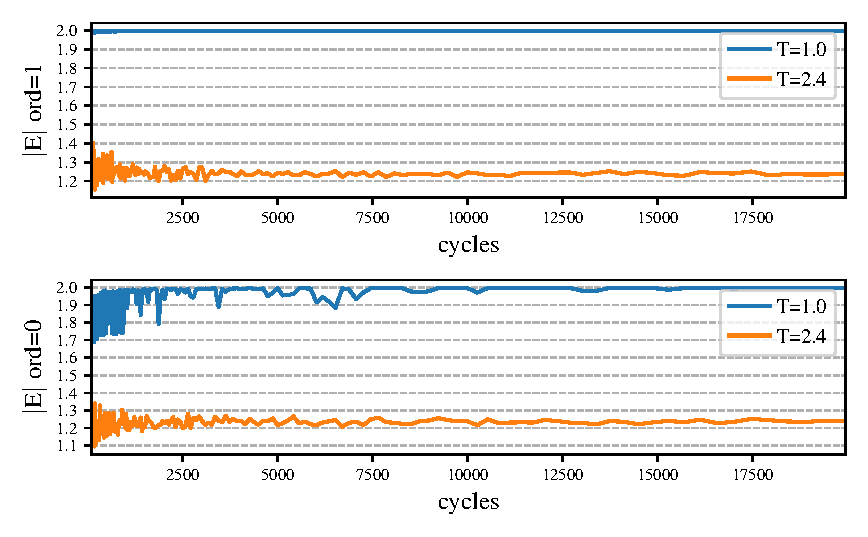
\includegraphics[width=0.8\textwidth]{../figures/equilibrium_E.pdf}
  \caption{Absolute values of energy for different MC cycles.
  ord refers to the initial microstate of spins. 1=up, 0=random.}
  \label{fig:equi_E}
\end{figure}


\begin{figure}[H]
  \centering
  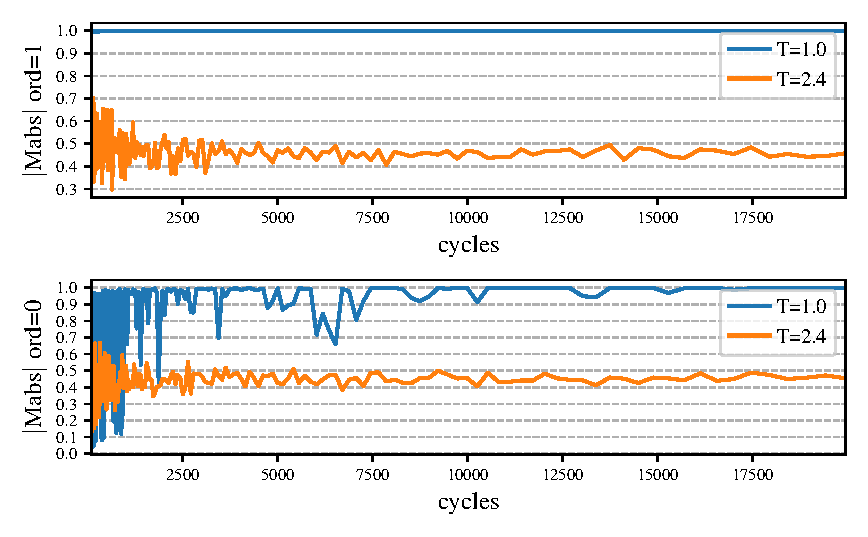
\includegraphics[width=0.8\textwidth]{../figures/equilibrium_Mabs.pdf}
  \caption{Absolute values of magnetization for different MC cycles.
  ord refers to the initial microstate of spins. 1=up, 0=random.}
  \label{fig:equi_M}
\end{figure}




\begin{figure}[H]
  \centering
  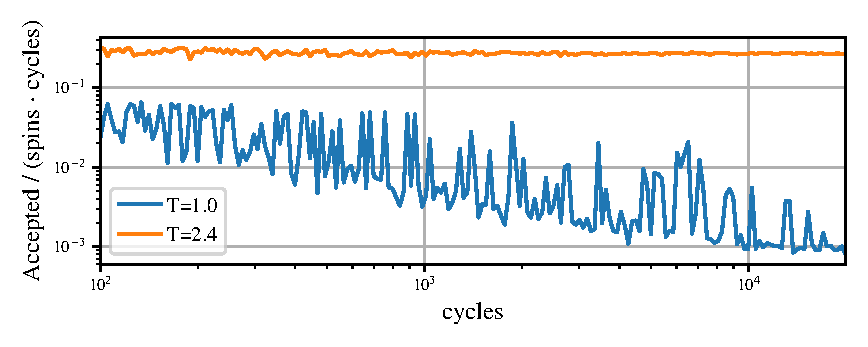
\includegraphics[width=\textwidth]{../figures/accepted.pdf}
  \caption{Accepted microstates scaled with number of spins and MC cycles.}
  \label{fig:accepted}
\end{figure}

\subsection{Model testing and error analysis}

Implementation of tests \footnote{test\_analytic.py, test\_ising.py} showed that the
analytical solutions was correct down to an absolute error of \num{1e-12}  when
comparing against a brute force method where we created all the possible
microstates.


To test the implementation of the ising model we calculated the relative error
in energy, magnetization, heat capacity and susceptibility (\cref{fig:error_L2})
for L=2 (where we have calculated analytical solutions). The relative error
was proportional to $1/ \sqrt \text{MC cycles}$. While there were some
differences in the relative error between the ordered and unordered inital
configuration for few Monte Carlo cycles, the difference decreased as we run more
cycles.

\begin{figure}[H]
  \centering
  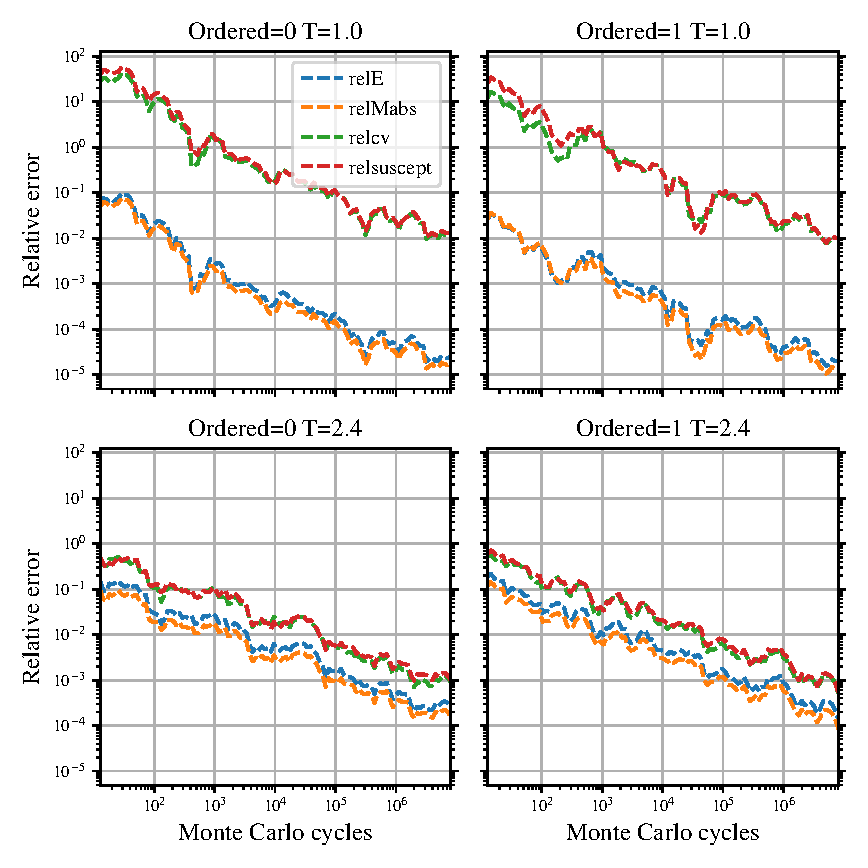
\includegraphics[width=\textwidth]{../figures/relative_error.pdf}
  \caption{Relative error vs MC cycles for L=2 for two different temperatures. Ordered
  refers to the inital spin configuration, with 1 meaning all spins pointing up and
  0 meaning a random configuration. Plots were smoothed by taking a
  rolling mean with window size 5. The relative error is proportional to
  $\frac{1}{\sqrt \text{MC cycles}}$.}
  \label{fig:error_L2}
\end{figure}


\subsection{Production runs}

The production runs (phase\_transitions.py) was parallelized using
$@njit(parallel=True)$ functionality within numba. It was easiest to run
calculations for each temperature in parallel, instead of parallelizing the
Ising model itself. A limitation of the using numba for parallelization was that
we were un able to write to file after each run of the Ising model. This made
our code vulnerable to crashes, since if the run
did not finish we would lose all the results. Timings with and without parallelization for small grid sizes showed a speedup
of roughly 3.4 on a computer with 4 physical cores.

To get a measure on how long the production runs would take, we created a script
\footnote{timings.py} that estimates the time to
run phase\_transitions.py with the given parameters, to avoid starting
too time consuming runs.

We did two production runs, one over a larger temperature range from $\beta \in
[2.0, 2.8]$ where aim we capture the larger picture, both before and after the
phase transition. Then the second run centred around the critical
temperature  $\beta \in [2.2, 2.35]$. Both runs was ran for four different grid
sizes $L \in [20,40,80,100]$, and with 1 million MC cycles, for which we
discarded the first 50000 samples. The temperature step size for the two runs
$dT$ was 0.001 and 0.0005 respectively. All production runs were started with
an unordered state.

\subsection{Probability distribution}

\begin{figure}[h]
  \begin{subfigure}[t]{\textwidth} % top align
    \centering
    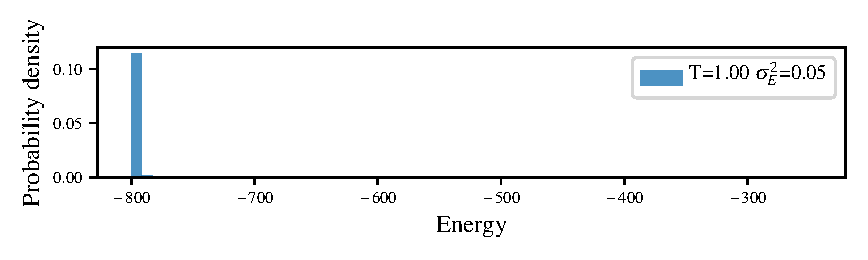
\includegraphics[width=\linewidth]{../figures/distribution_0.pdf}
    \caption{When the temperature is low $\sigma_E^2$ is also low and almost all
    of the energies are concentrated narrowly around the most likely
    state.}
    \label{fig:sub-first}
  \end{subfigure}
  \hfill
  \newline
  \begin{subfigure}[t]{\textwidth}
    \centering
    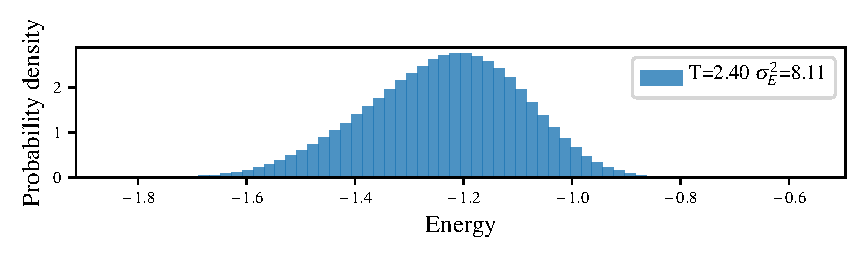
\includegraphics[width=\linewidth]{../figures/distribution_5.pdf}
    \caption{Higher temperature gives a higher $\sigma_E^2$ and fluctuations around
    the most likely state.}
    \label{fig:sub-second}
  \end{subfigure}
  \label{fig:distribution}
  \caption{Probability distribution of energy, scaled with number of spins. L=20
  MC cycles = \num{1e6}.}
\end{figure}


The probability distribution of energy (\cref{fig:distribution}) shows that
at low temperature almost all of the states are in a low energy state.
As the temperature and the variance increases the distribution becomes more
spread out.
